%!TEX root = ../../master.tex
\section{Experiment 1 - Learning Experience}
The following experiments are designed to qualify the effects of the designed course and the use of the Raspberry Pi cluster as a learning object to further highlighting the possible problems we introduce when introducing interprocess communication over a non-deterministic network.

\subsection*{Experiment 1.1 - Course}
In order to evaluate the impact of the chosen methods, we need to design experiments that will give insights into the progress of the teaching. 

\subsubsection*{Experiment 1.1.1: Determining students learning style}
\label{sec:exp1_1_1_learningstyle}
In order to target the learning experience, we need to understand how the students learn. Before beginning the learning activity, we need to determine how the students themselves rate their learning style. As described in Section~\ref{section:learning_styles}, Felder and Silverman describes four categories of learning styles. Felder further created a questionnaire to determine individual students preferred styles of leaning within the four categories. This questionnaire contains a total of 44 questions where the student must chose between two possible answers to each question. \\

\noindent In order to determining the students learning styles, an assignment is created before the class starts, where the students are asked to fill out the questionnaire and and in the results. The expected results of this experiment are to confirm the results of Felder and Silvermans research stating that engineering students are active, sensing, visual and sequential learners.\\

\noindent\textbf{Test protocol} \\
The test protocol involves sending out the questionnaire to each student, and have them answer the 44 questions and handing in the results. \\

\noindent\textbf{Metrics} \\
The questionnaire returns a result with a rating of your preferences in the four main categories. An example of this is seen in figure~\ref{fig:questionnaire}

\begin{figure}[H]
\centering
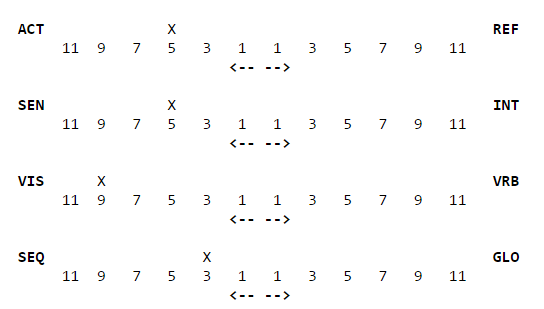
\includegraphics[scale=0.9]{figures/questionnaire_learning_style}
\caption{Example of the results of the questionnaire}
\label{fig:questionnaire}
\end{figure}


\noindent\textbf{Data basis}\\
The data basis consist of 16 engineering students. The students gender is all males and they are on their last year of their bachelor of information- and communication technology at Aarhus University School of Engineering. \\

\subsubsection*{Experiment 1.1.2: Determining the effects of learning activities on a weekly basis}

After determining the students learning style, we need to determine whether or not the students reach an adequate stage in SOLO's taxonomy. The course is designed around the weekly learning goals. In order to evaluate the students progression, a weekly reflection assignment is handed in. The goal of this reflection assignment is for the students to reflect upon the weeks learning activities and at the same time, provide insight in the students progression using SOLO's taxonomy. The assignment contains between 3 and 7 questions. The questions are all asked openly, and the students are provided with a textfield to input their thoughts. \\

\noindent\textbf{Test protocol}\\
The test protocol in this experiment consists of the time of when the questionnaires are released to the students. To ensure that the students answer the questionnaires they are mandetory for signing up for the exam. The questionnaires are released to the students in the last hour of the last lecture of every module. Below is the determined test protocol for each module.\\


\noindent\textit{Reflection before the course}\\

\vspace{-5mm}
\begin{enumerate}
	\setlength\itemsep{0.05em}
  \item What is cloud computing?
  \item What is a distributed system?
  \item What is cluster computing?
  \item What is virtualization?
  \item Describe some benefits and liabilities of sequential vs. parallel execution
  \item Describe your understanding of possible error in communicating over a network
  \item Describe your understanding of resilience in a system
\end{enumerate}

\noindent\textit{Module 1 - Course introduction, Cloud computing, frameworks}\\

\vspace{-5mm}
\begin{enumerate}
\setlength\itemsep{0.05em}
  \item What challenges do you see in cloud computing and microservice architecture?
  \item What would you say a cluster consist of?
  \item What benefits and drawbacks do you see in a microservice architecture compared to a monolithic architecture?
\end{enumerate}

\noindent\textit{Module 2 - Docker lightweight containers}\\

\vspace{-5mm}
\begin{enumerate}
\setlength\itemsep{0.05em}
  \item Describe with your own words the benefits and drawbacks of virtualization in general
  \item Describe with you own words, the difference between Containers and Virtual Machines on Hypervisors
  \item Describe with your own words, benefits and drawbacks of Docker containers
  \item Describe with your own words how Docker fits into a microservice architecture
\end{enumerate}


\noindent\textit{Module 3 - Kubernetes cluster manangement}\\

\vspace{-5mm}
\begin{enumerate}
\setlength\itemsep{0.05em}
	\item Describe the connection between Docker and Kubernetes
	\item Describe with your own words how Kubernetes orchestrates containers
	\item Describe with your own words the benefits and drawbacks of using a cluster management system such as Kubernetes
	\item How did workshop help you understand this week's topic
\end{enumerate}

\noindent\textit{Module 4 - Resilience and load testing}\\
TBD

\noindent\textit{Module 5 - Project work and external presentation}\\
TBD

\noindent\textit{Module 6 - Domain Name Service}\\
TBD

\noindent\textit{Module 7 - Service Discovery and project presentations}\\
TBD \\

\noindent\textbf{Metrics} \\
Since the questions are open-ended questions in their nature, the metrics will be of a qualitative nature. The goal is to get an insight in the students mental model, and quantify them using  SOLO's taxonomy. The metric in this case is a mapping between the answers and the learning goals of the module.\\

\noindent\textbf{Data basis} \\
The data basis consists of 17 male engineering students on the last year of their bachelor of information- and communication technology at Aarhus University School of Engineering. \\

\subsection*{Experiment 1.2 - Tangible cloud cluster}
\subsubsection*{Experiment 1.2.1 - Tangible cloud cluster as a learning object}
In order to determine if the Raspberry Pi cluster is a useful learning object, an experiment covering the students' experience with it and perception of it is designed. \\

\noindent The questionnaires from Experiment 1.1.2 are, in addition to validating the students' progress, designed to determine whether the cluster is useful as a learning object or not. Questions about the cluster's role are asked to disclose the students' mental models before, during and after the modules. The answers will be used to clarify the cluster's role as a learning object.

\subsubsection*{Test protocol}
  
\noindent The questions for the questionnaires are presented below. The questionnaires are sent out in the last hour of each module, except for the question for Module 1, which will be asked immediately after a demonstration of a Raspberry Pi cluster visualizing the benefit and drawbacks of distributing workloads in across multiple Raspberry Pis. This cluster is not the one used in the rest of the course, but a cluster from another project. \\

\noindent
\textit{Module 1}
\begin{enumerate}
\setlength\itemsep{0.05em}
	\item Did the cluster give you a better understanding of cluster computing?
\end{enumerate}

\noindent
\textit{Module 2 reflection}
\begin{enumerate}
\setlength\itemsep{0.05em}
	\item Describe how (if) the Raspberry Pi Cluster helped your learning
\end{enumerate}

\noindent
\textit{Module 3 reflection}
\begin{enumerate}
\setlength\itemsep{0.05em}
	\item Describe how (if) the Raspberry Pi Cluster helped your learning
	\item Describe how the Kubernetes visualization tool helped your learning
	\item How did the cluster help you understand the scheduling done by Kubernetes?
	\item How did the workshop help you understand this week's topic? 
\end{enumerate}

\noindent
\textit{Module 4 reflection}
\begin{enumerate}
\setlength\itemsep{0.05em}
	\item TBD
\end{enumerate}

\noindent
\textit{Module 5 reflection}
\begin{enumerate}
\setlength\itemsep{0.05em}
	\item TBD
\end{enumerate}

\noindent
\textit{Module 6 reflection}
\begin{enumerate}
\setlength\itemsep{0.05em}
	\item TBD
\end{enumerate}

\noindent
\textit{Module 7 reflection}
\begin{enumerate}
\setlength\itemsep{0.05em}
	\item TBD
\end{enumerate}

\subsubsection*{Metrics}
Since the questions are open-ended questions in their nature, the metrics will be of a qualitative nature.
\\
Statements from the students are expected to confirm the value of the cluster as a learning object and help to classify the type of learning object according to Churchill's classifications. The cluster's role as a mediating tool as described in activity theory is also expected to be seen from the answers. Lastly the importance of an object to explore and play with, as described by in constructivist learning theory, is expected to be observed in the students' answers.

\subsubsection*{Data basis}
The data basis consists of 16 male engineering students on the last year of their bachelor of information- and communication technology at Aarhus University School of Engineering.
